\documentclass[]{book}
\usepackage{lmodern}
\usepackage{amssymb,amsmath}
\usepackage{ifxetex,ifluatex}
\usepackage{fixltx2e} % provides \textsubscript
\ifnum 0\ifxetex 1\fi\ifluatex 1\fi=0 % if pdftex
  \usepackage[T1]{fontenc}
  \usepackage[utf8]{inputenc}
\else % if luatex or xelatex
  \ifxetex
    \usepackage{mathspec}
  \else
    \usepackage{fontspec}
  \fi
  \defaultfontfeatures{Ligatures=TeX,Scale=MatchLowercase}
\fi
% use upquote if available, for straight quotes in verbatim environments
\IfFileExists{upquote.sty}{\usepackage{upquote}}{}
% use microtype if available
\IfFileExists{microtype.sty}{%
\usepackage{microtype}
\UseMicrotypeSet[protrusion]{basicmath} % disable protrusion for tt fonts
}{}
\usepackage[margin=1.5in]{geometry}
\usepackage{hyperref}
\hypersetup{unicode=true,
            pdftitle={IQSS Workshops},
            pdfborder={0 0 0},
            breaklinks=true}
\urlstyle{same}  % don't use monospace font for urls
\usepackage{natbib}
\bibliographystyle{apalike}
\usepackage{color}
\usepackage{fancyvrb}
\newcommand{\VerbBar}{|}
\newcommand{\VERB}{\Verb[commandchars=\\\{\}]}
\DefineVerbatimEnvironment{Highlighting}{Verbatim}{commandchars=\\\{\}}
% Add ',fontsize=\small' for more characters per line
\usepackage{framed}
\definecolor{shadecolor}{RGB}{248,248,248}
\newenvironment{Shaded}{\begin{snugshade}}{\end{snugshade}}
\newcommand{\KeywordTok}[1]{\textcolor[rgb]{0.13,0.29,0.53}{\textbf{#1}}}
\newcommand{\DataTypeTok}[1]{\textcolor[rgb]{0.13,0.29,0.53}{#1}}
\newcommand{\DecValTok}[1]{\textcolor[rgb]{0.00,0.00,0.81}{#1}}
\newcommand{\BaseNTok}[1]{\textcolor[rgb]{0.00,0.00,0.81}{#1}}
\newcommand{\FloatTok}[1]{\textcolor[rgb]{0.00,0.00,0.81}{#1}}
\newcommand{\ConstantTok}[1]{\textcolor[rgb]{0.00,0.00,0.00}{#1}}
\newcommand{\CharTok}[1]{\textcolor[rgb]{0.31,0.60,0.02}{#1}}
\newcommand{\SpecialCharTok}[1]{\textcolor[rgb]{0.00,0.00,0.00}{#1}}
\newcommand{\StringTok}[1]{\textcolor[rgb]{0.31,0.60,0.02}{#1}}
\newcommand{\VerbatimStringTok}[1]{\textcolor[rgb]{0.31,0.60,0.02}{#1}}
\newcommand{\SpecialStringTok}[1]{\textcolor[rgb]{0.31,0.60,0.02}{#1}}
\newcommand{\ImportTok}[1]{#1}
\newcommand{\CommentTok}[1]{\textcolor[rgb]{0.56,0.35,0.01}{\textit{#1}}}
\newcommand{\DocumentationTok}[1]{\textcolor[rgb]{0.56,0.35,0.01}{\textbf{\textit{#1}}}}
\newcommand{\AnnotationTok}[1]{\textcolor[rgb]{0.56,0.35,0.01}{\textbf{\textit{#1}}}}
\newcommand{\CommentVarTok}[1]{\textcolor[rgb]{0.56,0.35,0.01}{\textbf{\textit{#1}}}}
\newcommand{\OtherTok}[1]{\textcolor[rgb]{0.56,0.35,0.01}{#1}}
\newcommand{\FunctionTok}[1]{\textcolor[rgb]{0.00,0.00,0.00}{#1}}
\newcommand{\VariableTok}[1]{\textcolor[rgb]{0.00,0.00,0.00}{#1}}
\newcommand{\ControlFlowTok}[1]{\textcolor[rgb]{0.13,0.29,0.53}{\textbf{#1}}}
\newcommand{\OperatorTok}[1]{\textcolor[rgb]{0.81,0.36,0.00}{\textbf{#1}}}
\newcommand{\BuiltInTok}[1]{#1}
\newcommand{\ExtensionTok}[1]{#1}
\newcommand{\PreprocessorTok}[1]{\textcolor[rgb]{0.56,0.35,0.01}{\textit{#1}}}
\newcommand{\AttributeTok}[1]{\textcolor[rgb]{0.77,0.63,0.00}{#1}}
\newcommand{\RegionMarkerTok}[1]{#1}
\newcommand{\InformationTok}[1]{\textcolor[rgb]{0.56,0.35,0.01}{\textbf{\textit{#1}}}}
\newcommand{\WarningTok}[1]{\textcolor[rgb]{0.56,0.35,0.01}{\textbf{\textit{#1}}}}
\newcommand{\AlertTok}[1]{\textcolor[rgb]{0.94,0.16,0.16}{#1}}
\newcommand{\ErrorTok}[1]{\textcolor[rgb]{0.64,0.00,0.00}{\textbf{#1}}}
\newcommand{\NormalTok}[1]{#1}
\usepackage{longtable,booktabs}
\usepackage{graphicx,grffile}
\makeatletter
\def\maxwidth{\ifdim\Gin@nat@width>\linewidth\linewidth\else\Gin@nat@width\fi}
\def\maxheight{\ifdim\Gin@nat@height>\textheight\textheight\else\Gin@nat@height\fi}
\makeatother
% Scale images if necessary, so that they will not overflow the page
% margins by default, and it is still possible to overwrite the defaults
% using explicit options in \includegraphics[width, height, ...]{}
\setkeys{Gin}{width=\maxwidth,height=\maxheight,keepaspectratio}
\IfFileExists{parskip.sty}{%
\usepackage{parskip}
}{% else
\setlength{\parindent}{0pt}
\setlength{\parskip}{6pt plus 2pt minus 1pt}
}
\setlength{\emergencystretch}{3em}  % prevent overfull lines
\providecommand{\tightlist}{%
  \setlength{\itemsep}{0pt}\setlength{\parskip}{0pt}}
\setcounter{secnumdepth}{5}
% Redefines (sub)paragraphs to behave more like sections
\ifx\paragraph\undefined\else
\let\oldparagraph\paragraph
\renewcommand{\paragraph}[1]{\oldparagraph{#1}\mbox{}}
\fi
\ifx\subparagraph\undefined\else
\let\oldsubparagraph\subparagraph
\renewcommand{\subparagraph}[1]{\oldsubparagraph{#1}\mbox{}}
\fi

%%% Use protect on footnotes to avoid problems with footnotes in titles
\let\rmarkdownfootnote\footnote%
\def\footnote{\protect\rmarkdownfootnote}

%%% Change title format to be more compact
\usepackage{titling}

% Create subtitle command for use in maketitle
\providecommand{\subtitle}[1]{
  \posttitle{
    \begin{center}\large#1\end{center}
    }
}

\setlength{\droptitle}{-2em}

  \title{IQSS Workshops}
    \pretitle{\vspace{\droptitle}\centering\huge}
  \posttitle{\par}
    \author{}
    \preauthor{}\postauthor{}
      \predate{\centering\large\emph}
  \postdate{\par}
    \date{September 2019}

\usepackage{booktabs}

\usepackage{epsfig}
\usepackage{epstopdf}
\usepackage{rotate}
\usepackage{graphicx}
\usepackage{hyperref}
\usepackage{alphalph}
\usepackage{caption}
\usepackage[hang,flushmargin]{footmisc}
\usepackage{framed}
\usepackage{xcolor}
\usepackage{verbatim} 

\usepackage{bm}
\setcounter{MaxMatrixCols}{20}
\newcommand{\Var}{\mathrm{Var}}
\newcommand{\SD}{\mathrm{SD}}
\newcommand{\Cov}{\mathrm{Cov}}
\newcommand{\fx}{f({\bf x})}
\newcommand\R{{\textsf R~}}
\newcommand\Rst{\textsf{RStudio}}

% spacing between environments
\usepackage{amsthm}
\makeatletter
\def\thm@space@setup{%
  \thm@preskip=15pt plus 2pt minus 4pt
  \thm@postskip=\thm@preskip
}
\makeatother


% Title format
\usepackage{titling}
\pretitle{\Huge\sffamily}
\posttitle{\par\vskip 0.5em}
\predate{\LARGE\sffamily}
\postdate{\par}

\urlstyle{tt}

\begin{document}
\maketitle

{
\setcounter{tocdepth}{1}
\tableofcontents
}
\chapter*{Introduction}\label{introduction}
\addcontentsline{toc}{chapter}{Introduction}

\section*{Table of Contents}\label{table-of-contents}
\addcontentsline{toc}{section}{Table of Contents}

Materials for the \href{http://dss.iq.harvard.edu}{Data Science
Services} statistical software workshops from the
\href{http://iq.harvard.edu}{Institute for Quantitative Social Science}
at Harvard.

\begin{enumerate}
\def\labelenumi{\arabic{enumi}.}
\tightlist
\item
  \href{./R/Rintro/Rintro.html}{Introduction to R}
\item
  \href{./R/Rmodels/Rmodels.html}{Regression models in R}
\item
  \href{./R/Rgraphics/Rgraphics.html}{Graphics in R using ggplot2}
\item
  \href{./R/RDataWrangling/RDataWrangling.html}{R data wrangling}
\item
  \href{./Python/PythonIntro/PythonIntro.html}{Introduction to Python}
\item
  \href{./Python/PythonWebScrape/PythonWebScrape.html}{Python
  web-scraping}
\item
  \href{./Stata/StataIntro/StataIntro.html}{Introduction to Stata}
\end{enumerate}

These workshops are a work-in-progress, please provide feedback! Email:
\href{mailto:help@iq.harvard.edu}{\nolinkurl{help@iq.harvard.edu}}

\section*{Authors and Sources}\label{authors-and-sources}
\addcontentsline{toc}{section}{Authors and Sources}

These content of these workshops are almost entirely the work of Ista
Zahn, now at Harvard's School of Public Health. The current workshop
materials have been modified by Steve Worthington, Jinjie Liu, and Yihan
Wang, at Harvard's Institute for Quantitative Social Science.

\part{R}\label{part-r}

\chapter{Welcome}\label{welcome}

\textbf{Topics} Assignment; Function arguments; Finding help; Reading
data; Filtering and arranging data; Conditional operations; Saving data.

\section{Materials and setup}\label{materials-and-setup}

\textbf{NOTE: skip this section if you are not running R locally} (e.g.,
if you are running R in your browser using a remote Jupyter server)

You should have R installed --if not:

\begin{itemize}
\tightlist
\item
  Download and install R from \url{http://cran.r-project.org}
\item
  Download and install RStudio from
  \url{https://www.rstudio.com/products/rstudio/download/\#download}
\end{itemize}

Notes and examples for this workshop are available at
\href{http://tutorials.iq.harvard.edu/R/Rintro/Rintro.html}{}

Start RStudio create a new project: - On Windows click the start button
and search for rstudio. On Mac RStudio will be in your applications
folder. - In Rstudio go to \texttt{File\ -\textgreater{}\ New\ Project}.
- Choose \texttt{New\ Directory} and \texttt{New\ Project}. - Choose a
name and location for your new project directory.

\section{Workshop goals and approach}\label{workshop-goals-and-approach}

In this workshop you will

\begin{itemize}
\tightlist
\item
  learn R basics,
\item
  learn about the R package ecosystem,
\item
  practice reading files and manipulating data in R
\end{itemize}

A more general goal is to get you comfortable with R so that it seems
less scary and mystifying than it perhaps does now. Note that this is by
no means a complete or thorough introduction to R! It's just enough to
get you started.

This workshop is relatively informal, example-oriented, and hands-on. We
won't spend much time examining language features in detail. Instead we
will work through an example, and learn some things about the R along
the way.

As an example project we will analyze the popularity of baby names in
the US from 1960 through 2017. Among the questions we will use R to
answer are:

\begin{itemize}
\tightlist
\item
  In which year did your name achieve peak popularity?
\item
  How many children were born each year?
\item
  What are the most popular names overall? For girls? For Boys?
\end{itemize}

\chapter{Graphical User Interfaces
(GUIs)}\label{graphical-user-interfaces-guis}

There are many different ways you can interact with R. See the
\href{http://tutorials.iq.harvard.edu/DataScienceTools/DataScienceTools.html}{Data
Science Tools workshop notes} for details.

For this workshop I encourage you to use RStudio; it is a good
R-specific IDE that mostly just works.

\section{Launch RStudio (skip if not using
Rstudio)}\label{launch-rstudio-skip-if-not-using-rstudio}

\textbf{Note: skip this section if you are not using Rstudio (e.g., if
you are running these examples in a Jupyter notebook).}

\begin{itemize}
\tightlist
\item
  Start the RStudio program
\item
  In RStudio, go to \textbf{File =\textgreater{} New File
  =\textgreater{} R Script}
\end{itemize}

The window in the upper-left is your R script. This is where you will
write instructions for R to carry out.

The window in the lower-left is the R console. This is where results
will be displayed.

\section{Exercise 0}\label{exercise-0}

The purpose of this exercise is to give you an opportunity to explore
the interface provided by RStudio (or whichever GUI you've decided to
use). You may not know how to do these things; that's fine! This is an
opportunity to figure it out.

Also keep in mind that we are living in a golden age of tab completion.
If you don't know the name of an R function, try guessing the first two
or three letters and pressing TAB. If you guessed correctly the function
you are looking for should appear in a pop up!

\begin{center}\rule{0.5\linewidth}{\linethickness}\end{center}

\begin{enumerate}
\def\labelenumi{\arabic{enumi}.}
\tightlist
\item
  Try to get R to add 2 plus 2.
\end{enumerate}

\begin{Shaded}
\begin{Highlighting}[]
\NormalTok{##}
\end{Highlighting}
\end{Shaded}

\begin{enumerate}
\def\labelenumi{\arabic{enumi}.}
\setcounter{enumi}{1}
\tightlist
\item
  Try to calculate the square root of 10.
\end{enumerate}

\begin{Shaded}
\begin{Highlighting}[]
\NormalTok{##}
\end{Highlighting}
\end{Shaded}

\begin{enumerate}
\def\labelenumi{\arabic{enumi}.}
\setcounter{enumi}{2}
\tightlist
\item
  R includes extensive documentation, including a manual named ``An
  introduction to R''. Use the RStudio help pane. to locate this manual.
\end{enumerate}

\section{Exercise 0 solution}\label{exercise-0-solution}

\begin{Shaded}
\begin{Highlighting}[]
\NormalTok{## 1. 2 plus 2}
\DecValTok{2} \OperatorTok{+}\StringTok{ }\DecValTok{2}
\NormalTok{## or}
\KeywordTok{sum}\NormalTok{(}\DecValTok{2}\NormalTok{, }\DecValTok{2}\NormalTok{)}
\end{Highlighting}
\end{Shaded}

\begin{Shaded}
\begin{Highlighting}[]
\NormalTok{## 2. square root of 10:}
\KeywordTok{sqrt}\NormalTok{(}\DecValTok{10}\NormalTok{)}
\NormalTok{## or}
\DecValTok{10}\OperatorTok{^}\NormalTok{(}\DecValTok{1}\OperatorTok{/}\DecValTok{2}\NormalTok{)}
\end{Highlighting}
\end{Shaded}

\begin{Shaded}
\begin{Highlighting}[]
\NormalTok{## 3. Find "An Introduction to R".}
\end{Highlighting}
\end{Shaded}

\begin{Shaded}
\begin{Highlighting}[]
\NormalTok{## Go to the main help page by running 'help.start() or using the GUI}
\NormalTok{## menu, find and click on the link to "An Introduction to R".}
\end{Highlighting}
\end{Shaded}

\chapter{R basics}\label{r-basics}

\section{Function calls}\label{function-calls}

The general form for calling R functions is

\begin{Shaded}
\begin{Highlighting}[]
\NormalTok{## FunctionName(arg.1 = value.1, arg.2 = value.2, ..., arg.n - value.n)}
\end{Highlighting}
\end{Shaded}

Arguments can be matched by name; unnamed arguments will be matched by
position.

\section{Assignment}\label{assignment}

Values can be assigned names and used in subsequent operations

\begin{itemize}
\tightlist
\item
  The ``gets'' \texttt{\textless{}-} operator (less than followed by a
  dash) is used to save values
\item
  The name on the left gets the value on the right.
\end{itemize}

\begin{Shaded}
\begin{Highlighting}[]
\KeywordTok{sqrt}\NormalTok{(}\DecValTok{10}\NormalTok{) ## calculate square root of 10; result is not stored anywhere}
\NormalTok{x <-}\StringTok{ }\KeywordTok{sqrt}\NormalTok{(}\DecValTok{10}\NormalTok{) }\CommentTok{# assign result to a variable named x}
\end{Highlighting}
\end{Shaded}

Names should start with a letter, and contain only letters, numbers,
underscores, and periods.

\section{Asking R for help}\label{asking-r-for-help}

You can ask R for help using the \texttt{help} function, or the
\texttt{?} shortcut.

\begin{Shaded}
\begin{Highlighting}[]
\KeywordTok{help}\NormalTok{(help)}
\end{Highlighting}
\end{Shaded}

The \texttt{help} function can be used to look up the documentation for
a function, or to look up the documentation to a package. We can learn
how to use the \texttt{stats} package by reading its documentation like
this:

\begin{Shaded}
\begin{Highlighting}[]
\KeywordTok{help}\NormalTok{(}\DataTypeTok{package =} \StringTok{"stats"}\NormalTok{)}
\end{Highlighting}
\end{Shaded}

\chapter{Getting data into R}\label{getting-data-into-r}

R has data reading functionality built-in -- see e.g.,
\texttt{help(read.table)}. However, faster and more robust tools are
available, and so to make things easier on ourselves we will use a
\emph{contributed package} called \texttt{readr} instead. This requires
that we learn a little bit about packages in R.

\section{Installing and using R
packages}\label{installing-and-using-r-packages}

A large number of contributed packages are available. If you are looking
for a package for a specific task,
\url{https://cran.r-project.org/web/views/} and \url{https://r-pkg.org}
are good places to start.

You can install a package in R using the \texttt{install.packages()}
function. Once a package is installed you may use the \texttt{library}
function to attach it so that it can be used.

\begin{Shaded}
\begin{Highlighting}[]
\NormalTok{## install.packages("readr")}
\KeywordTok{library}\NormalTok{(readr)}
\end{Highlighting}
\end{Shaded}

\section{Readers for common file
types}\label{readers-for-common-file-types}

In order to read data from a file, you have to know what kind of file it
is. The table below lists functions that can import data from common
plain-text formats.

\begin{longtable}[]{@{}ll@{}}
\toprule
Data Type & Function\tabularnewline
\midrule
\endhead
comma separated & \texttt{read\_csv()}\tabularnewline
tab separated & \texttt{read\_delim()}\tabularnewline
other delimited formats & \texttt{read\_table()}\tabularnewline
fixed width & \texttt{read\_fwf()}\tabularnewline
\bottomrule
\end{longtable}

\textbf{Note} You may be confused by the existence of similar functions,
e.g., \texttt{read.csv} and \texttt{read.delim}. These are legacy
functions that tend to be slower and less robust than the \texttt{readr}
functions. One way to tell them apart is that the faster more robust
versions use underscores in their names (e.g., \texttt{read\_csv}) while
the older functions us dots (e.g., \texttt{read.csv}). My advice is to
use the more robust newer versions, i.e., the ones with underscores.

\section{Baby names data}\label{baby-names-data}

The examples in this workshop use US baby names data retrieved from
\url{https://catalog.data.gov/dataset/baby-names-from-social-security-card-applications-national-level-data}
A cleaned and merged version of these data is available at
\texttt{http://tutorials.iq.harvard.edu/data/babyNames.csv}.

\section{Exercise 1: Reading the baby names
data}\label{exercise-1-reading-the-baby-names-data}

Make sure you have installed the \texttt{readr} package and attached it
with \texttt{library(readr)}.

Baby names data are available at
\texttt{"http://tutorials.iq.harvard.edu/data/babyNames.csv"}.

\begin{enumerate}
\def\labelenumi{\arabic{enumi}.}
\item
  Open the \texttt{read\_csv} help page to determine how to use it to
  read in data.
\item
  Read the baby names data using the \texttt{read\_csv} function and
  assign the result with the name \texttt{baby.names}.
\item
  BONUS (optional): Save the \texttt{baby.names} data as a Stata data
  set \texttt{babynames.dta} and as an R data set
  \texttt{babynames.rds}.
\end{enumerate}

\section{Exercise 1 solution}\label{exercise-1-solution}

\begin{Shaded}
\begin{Highlighting}[]
\NormalTok{## read ?read_csv}
\end{Highlighting}
\end{Shaded}

\begin{Shaded}
\begin{Highlighting}[]
\NormalTok{baby.names <-}\StringTok{ }\KeywordTok{read_csv}\NormalTok{(}\StringTok{"http://tutorials.iq.harvard.edu/data/babyNames.csv"}\NormalTok{)}
\end{Highlighting}
\end{Shaded}

\chapter{Popularity of your name}\label{popularity-of-your-name}

In this section we will pull out specific names and examine changes in
their popularity over time.

The \texttt{baby.names} object we created in the last exercise is a
\texttt{data.frame}. There are many other data structures in R, but for
now we'll focus on working with \texttt{data.frames}.

R has decent data manipulation tools built-in -- see e.g.,
\texttt{help(Extract)}. However, these tools are powerful and complex
and often overwhelm beginners. To make things easier on ourselves we
will use a \emph{contributed package} called \texttt{dplyr} instead.

\begin{Shaded}
\begin{Highlighting}[]
\NormalTok{## install.packages("dplyr")}
\KeywordTok{library}\NormalTok{(dplyr)}
\end{Highlighting}
\end{Shaded}

\section{Filtering and arranging
data}\label{filtering-and-arranging-data}

One way to find the year in which your name was the most popular is to
filter out just the rows corresponding to your name, and then arrange
(sort) by Count.

To demonstrate these techniques we'll try to determine whether ``Alex''"
or ``Jim'' was more popular in 1992. We start by filtering the data so
that we keep only rows where Year is equal to \texttt{1992} and Name is
either ``Alex'' or ``Mark''.

\begin{Shaded}
\begin{Highlighting}[]
\NormalTok{am <-}\StringTok{ }\KeywordTok{filter}\NormalTok{(baby.names, }
\NormalTok{             Year }\OperatorTok{==}\StringTok{ }\DecValTok{1992} \OperatorTok{&}\StringTok{ }\NormalTok{(Name }\OperatorTok{==}\StringTok{ "Alex"} \OperatorTok{|}\StringTok{ }\NormalTok{Name }\OperatorTok{==}\StringTok{ "Mark"}\NormalTok{))}
\NormalTok{am}
\end{Highlighting}
\end{Shaded}

Notice that we can we can combine conditons using \texttt{\&} (AND) and
\texttt{\textbar{}} (OR).

In this case it's pretty easy to see that ``Mark'' is more popular, but
to make it even easier we can arrange the data so that the most popular
name is listed first.

\begin{Shaded}
\begin{Highlighting}[]
\KeywordTok{arrange}\NormalTok{(am, Count)}
\end{Highlighting}
\end{Shaded}

\begin{Shaded}
\begin{Highlighting}[]
\KeywordTok{arrange}\NormalTok{(am, }\KeywordTok{desc}\NormalTok{(Count))}
\end{Highlighting}
\end{Shaded}

\section{Other logical operators}\label{other-logical-operators}

In the previous example we used \texttt{==} to filter rows. Other
relational and logical operators are listed below.

\begin{longtable}[]{@{}ll@{}}
\toprule
Operator & Meaning\tabularnewline
\midrule
\endhead
\texttt{==} & equal to\tabularnewline
\texttt{!=} & not equal to\tabularnewline
\texttt{\textgreater{}} & greater than\tabularnewline
\texttt{\textgreater{}=} & greater than or equal to\tabularnewline
\texttt{\textless{}} & less than\tabularnewline
\texttt{\textless{}=} & less than or equal to\tabularnewline
\texttt{\%in\%} & contained in\tabularnewline
\bottomrule
\end{longtable}

These operators may be combined with \texttt{\&} (and) or
\texttt{\textbar{}} (or).

\section{Exercise 2: Peak popularity of your
name}\label{exercise-2-peak-popularity-of-your-name}

In this exercise you will discover the year your name reached its
maximum popularity.

Read in the ``babyNames.csv'' file if you have not already done so,
assigning the result to \texttt{baby.names}. The file is located at
\texttt{"http://tutorials.iq.harvard.edu/data/babyNames.csv"}

Make sure you have installed the \texttt{dplyr} package and attached it
with \texttt{library(dplyr)}.

\begin{enumerate}
\def\labelenumi{\arabic{enumi}.}
\tightlist
\item
  Use \texttt{filter} to extract data for your name (or another name of
  your choice).
\end{enumerate}

\begin{Shaded}
\begin{Highlighting}[]
\NormalTok{##}
\end{Highlighting}
\end{Shaded}

\begin{enumerate}
\def\labelenumi{\arabic{enumi}.}
\setcounter{enumi}{1}
\tightlist
\item
  Arrange the data you produced in step 1 above by \texttt{Count}. In
  which year was the name most popular?
\end{enumerate}

\begin{Shaded}
\begin{Highlighting}[]
\NormalTok{##}
\end{Highlighting}
\end{Shaded}

\begin{enumerate}
\def\labelenumi{\arabic{enumi}.}
\setcounter{enumi}{2}
\tightlist
\item
  BONUS (optional): Filter the data to extract \emph{only} the row
  containing the most popular boys name in 1999.
\end{enumerate}

\begin{Shaded}
\begin{Highlighting}[]
\NormalTok{##}
\end{Highlighting}
\end{Shaded}

\section{Exercise 2 solution}\label{exercise-2-solution}

\begin{Shaded}
\begin{Highlighting}[]
\CommentTok{# 1.  Use `filter` to extract data for your name (or another name of your choice).  }
\end{Highlighting}
\end{Shaded}

\begin{Shaded}
\begin{Highlighting}[]
\NormalTok{george <-}\StringTok{ }\KeywordTok{filter}\NormalTok{(baby.names, Name }\OperatorTok{==}\StringTok{ "George"}\NormalTok{)}
\end{Highlighting}
\end{Shaded}

\begin{Shaded}
\begin{Highlighting}[]
\CommentTok{# 2.  Arrange the data you produced in step 1 above by `Count`. }
\CommentTok{#     In which year was the name most popular?}
\end{Highlighting}
\end{Shaded}

\begin{Shaded}
\begin{Highlighting}[]
\KeywordTok{arrange}\NormalTok{(george, }\KeywordTok{desc}\NormalTok{(Count))}
\end{Highlighting}
\end{Shaded}

\begin{Shaded}
\begin{Highlighting}[]
\CommentTok{# 3.  BONUS (optional): Filter the data to extract _only_ the }
\CommentTok{#     row containing the most popular boys name in 1999.}
\end{Highlighting}
\end{Shaded}

\begin{Shaded}
\begin{Highlighting}[]
\NormalTok{boys.}\DecValTok{1999}\NormalTok{ <-}\StringTok{ }\KeywordTok{filter}\NormalTok{(baby.names, }
\NormalTok{                    Year }\OperatorTok{==}\StringTok{ }\DecValTok{1999} \OperatorTok{&}\StringTok{ }\NormalTok{Sex }\OperatorTok{==}\StringTok{ "Boys"}\NormalTok{)}
\end{Highlighting}
\end{Shaded}

\begin{Shaded}
\begin{Highlighting}[]
\KeywordTok{filter}\NormalTok{(boys.}\DecValTok{1999}\NormalTok{, Count }\OperatorTok{==}\StringTok{ }\KeywordTok{max}\NormalTok{(Count))}
\end{Highlighting}
\end{Shaded}

\chapter{Plotting baby name trends over
time}\label{plotting-baby-name-trends-over-time}

It can be difficult to spot trends when looking at summary tables.
Plotting the data makes it easier to identify interesting patterns.

R has decent plotting tools built-in -- see e.g., \texttt{help(plot)}.
However, To make things easier on ourselves we will use a
\emph{contributed package} called \texttt{ggplot2} instead.

\begin{Shaded}
\begin{Highlighting}[]
\NormalTok{## install.packages("ggplot2")}
\KeywordTok{library}\NormalTok{(ggplot2)}
\end{Highlighting}
\end{Shaded}

For quick and simple plots we can use the \texttt{qplot} function. For
example, we can plot the number of babies given the name ``Diana'' over
time like this:

\begin{Shaded}
\begin{Highlighting}[]
\NormalTok{diana <-}\StringTok{ }\KeywordTok{filter}\NormalTok{(baby.names, Name }\OperatorTok{==}\StringTok{ "Diana"}\NormalTok{)}
\end{Highlighting}
\end{Shaded}

\begin{Shaded}
\begin{Highlighting}[]
\KeywordTok{qplot}\NormalTok{(}\DataTypeTok{x =}\NormalTok{ Year, }\DataTypeTok{y =}\NormalTok{ Count,}
     \DataTypeTok{data =}\NormalTok{ diana)}
\end{Highlighting}
\end{Shaded}

Interetingly there are usually some gender-atypical names, even for very
strongly gendered names like ``Diana''. Splitting these trends out by
Sex is very easy:

\begin{Shaded}
\begin{Highlighting}[]
\KeywordTok{qplot}\NormalTok{(}\DataTypeTok{x =}\NormalTok{ Year, }\DataTypeTok{y =}\NormalTok{ Count, }\DataTypeTok{color =}\NormalTok{ Sex,}
      \DataTypeTok{data =}\NormalTok{ diana)}
\end{Highlighting}
\end{Shaded}

\section{Exercise 3: Plotting peak popularity of your
name}\label{exercise-3-plotting-peak-popularity-of-your-name}

Make sure the \texttt{ggplot2} package is installed, and that you have
attached it using \texttt{library(ggplot2)}.

\begin{enumerate}
\def\labelenumi{\arabic{enumi}.}
\tightlist
\item
  Use \texttt{filter} to extract data for your name (same as previous
  exercise)
\end{enumerate}

\begin{Shaded}
\begin{Highlighting}[]
\NormalTok{##}
\end{Highlighting}
\end{Shaded}

\begin{enumerate}
\def\labelenumi{\arabic{enumi}.}
\setcounter{enumi}{1}
\tightlist
\item
  Plot the data you produced in step 1 above, with \texttt{Year} on the
  x-axis and \texttt{Count} on the y-axis.
\end{enumerate}

\begin{Shaded}
\begin{Highlighting}[]
\NormalTok{##}
\end{Highlighting}
\end{Shaded}

\begin{enumerate}
\def\labelenumi{\arabic{enumi}.}
\setcounter{enumi}{2}
\tightlist
\item
  Adjust the plot so that is shows boys and girls in different colors.
\end{enumerate}

\begin{Shaded}
\begin{Highlighting}[]
\NormalTok{##}
\end{Highlighting}
\end{Shaded}

\begin{enumerate}
\def\labelenumi{\arabic{enumi}.}
\setcounter{enumi}{3}
\tightlist
\item
  BONUS (Optional): Adust the plot to use lines instead of points.
\end{enumerate}

\section{Exercise 3 solution}\label{exercise-3-solution}

\begin{Shaded}
\begin{Highlighting}[]
\CommentTok{# 1. Use `filter` to extract data for your name (same as previous exercise)  }
\end{Highlighting}
\end{Shaded}

\begin{Shaded}
\begin{Highlighting}[]
\NormalTok{george <-}\StringTok{ }\KeywordTok{filter}\NormalTok{(baby.names, Name }\OperatorTok{==}\StringTok{ "George"}\NormalTok{)}
\end{Highlighting}
\end{Shaded}

\begin{Shaded}
\begin{Highlighting}[]
\CommentTok{# 2.  Plot the data you produced in step 1 above, with `Year` on the x-axis}
\CommentTok{#     and `Count` on the y-axis.}
\end{Highlighting}
\end{Shaded}

\begin{Shaded}
\begin{Highlighting}[]
\KeywordTok{qplot}\NormalTok{(}\DataTypeTok{x =}\NormalTok{ Year, }\DataTypeTok{y =}\NormalTok{ Count, }\DataTypeTok{data =}\NormalTok{ george)}
\end{Highlighting}
\end{Shaded}

\begin{Shaded}
\begin{Highlighting}[]
\CommentTok{# 3. Adjust the plot so that is shows boys and girls in different colors.}
\end{Highlighting}
\end{Shaded}

\begin{Shaded}
\begin{Highlighting}[]
\KeywordTok{qplot}\NormalTok{(}\DataTypeTok{x =}\NormalTok{ Year, }\DataTypeTok{y =}\NormalTok{ Count, }\DataTypeTok{color =}\NormalTok{ Sex, }\DataTypeTok{data =}\NormalTok{ george)}
\end{Highlighting}
\end{Shaded}

\begin{Shaded}
\begin{Highlighting}[]
\CommentTok{# 4.  BONUS (Optional): Adust the plot to use lines instead of points.}
\end{Highlighting}
\end{Shaded}

\begin{Shaded}
\begin{Highlighting}[]
\KeywordTok{qplot}\NormalTok{(}\DataTypeTok{x =}\NormalTok{ Year, }\DataTypeTok{y =}\NormalTok{ Count, }\DataTypeTok{color =}\NormalTok{ Sex, }\DataTypeTok{data =}\NormalTok{ george, }\DataTypeTok{geom =} \StringTok{"line"}\NormalTok{)}
\end{Highlighting}
\end{Shaded}

\chapter{Finding the most popular
names}\label{finding-the-most-popular-names}

Our next goal is to find out which names have been the most popular.

\section{Computing better measures of
popularity}\label{computing-better-measures-of-popularity}

So far we've used \texttt{Count} as a measure of popularity. A better
approach is to use proportion or rank to avoid confounding popularity
with the number of babies born in a given year.

The \texttt{mutate} function makes it easy to add or modify the columns
of a \texttt{data.frame}. For example, we can use it compute the log of
the number of boys and girls given each name in each year:

\begin{Shaded}
\begin{Highlighting}[]
\NormalTok{baby.names <-}\StringTok{ }\KeywordTok{mutate}\NormalTok{(baby.names, }\DataTypeTok{logCount =}\NormalTok{ Count}\OperatorTok{/}\DecValTok{1000}\NormalTok{)}
\NormalTok{baby.names}
\end{Highlighting}
\end{Shaded}

\section{Operating by group}\label{operating-by-group}

Because of the nested nature of out data, we want to compute rank or
proportion within each \texttt{Sex} \texttt{X} \texttt{Year} group. The
\texttt{dplyr} package makes this relatively easy.

\begin{Shaded}
\begin{Highlighting}[]
\NormalTok{baby.names <-}\StringTok{ }\KeywordTok{mutate}\NormalTok{(}\KeywordTok{group_by}\NormalTok{(baby.names, Year, Sex),}
                     \DataTypeTok{Rank =} \KeywordTok{rank}\NormalTok{(Count))}
\end{Highlighting}
\end{Shaded}

Note that the data remains grouped until you change the groups by
running \texttt{group\_by} again or remove grouping information with
\texttt{ungroup}.

\section{Exercise 4: Most popular
names}\label{exercise-4-most-popular-names}

In this exercise your goal is to identify the most popular names for
each year.

\begin{enumerate}
\def\labelenumi{\arabic{enumi}.}
\tightlist
\item
  Use \texttt{mutate} and \texttt{group\_by} to create a column named
  ``Proportion'' where \texttt{Proportion\ =\ Count/sum(Count)} for each
  \texttt{Year\ X\ Sex} group.
\end{enumerate}

\begin{Shaded}
\begin{Highlighting}[]
\NormalTok{##}
\end{Highlighting}
\end{Shaded}

\begin{enumerate}
\def\labelenumi{\arabic{enumi}.}
\setcounter{enumi}{1}
\tightlist
\item
  Use \texttt{mutate} and \texttt{group\_by} to create a column named
  ``Rank'' where \texttt{Rank\ =\ rank(-Count)} for each
  \texttt{Year\ X\ Sex} group.
\end{enumerate}

\begin{Shaded}
\begin{Highlighting}[]
\NormalTok{##}
\end{Highlighting}
\end{Shaded}

\begin{enumerate}
\def\labelenumi{\arabic{enumi}.}
\setcounter{enumi}{2}
\tightlist
\item
  Filter the baby names data to display only the most popular name for
  each \texttt{Year\ X\ Sex} group.
\end{enumerate}

\begin{Shaded}
\begin{Highlighting}[]
\NormalTok{##}
\end{Highlighting}
\end{Shaded}

\begin{enumerate}
\def\labelenumi{\arabic{enumi}.}
\setcounter{enumi}{3}
\tightlist
\item
  Plot the data produced in step 4, putting \texttt{Year} on the x-axis
  and \texttt{Proportion} on the y-axis. How has the proportion of
  babies given the most popular name changed over time?
\end{enumerate}

\begin{Shaded}
\begin{Highlighting}[]
\NormalTok{##}
\end{Highlighting}
\end{Shaded}

\begin{enumerate}
\def\labelenumi{\arabic{enumi}.}
\setcounter{enumi}{4}
\tightlist
\item
  BONUS (optional): Which names are the most popular for both boys and
  girls?
\end{enumerate}

\section{Exercise 4 solution}\label{exercise-4-solution}

\begin{Shaded}
\begin{Highlighting}[]
\NormalTok{## 1.  Use `mutate` and `group_by` to create a column named "Proportion"}
\NormalTok{##     where `Proportion = Count/sum(Count)` for each `Year X Sex` group.}
\end{Highlighting}
\end{Shaded}

\begin{Shaded}
\begin{Highlighting}[]
\NormalTok{baby.names <-}\StringTok{ }\KeywordTok{mutate}\NormalTok{(}\KeywordTok{group_by}\NormalTok{(baby.names, Year, Sex),}
                     \DataTypeTok{Proportion =}\NormalTok{ Count}\OperatorTok{/}\KeywordTok{sum}\NormalTok{(Count))}
\end{Highlighting}
\end{Shaded}

\begin{Shaded}
\begin{Highlighting}[]
\NormalTok{## 2.  Use `mutate` and `group_by` to create a column named "Rank" where }
\NormalTok{##     `Rank = rank(-Count)` for each `Year X Sex` group.}
\end{Highlighting}
\end{Shaded}

\begin{Shaded}
\begin{Highlighting}[]
\NormalTok{baby.names <-}\StringTok{ }\KeywordTok{mutate}\NormalTok{(}\KeywordTok{group_by}\NormalTok{(baby.names, Year, Sex),}
                     \DataTypeTok{Rank =} \KeywordTok{rank}\NormalTok{(}\OperatorTok{-}\NormalTok{Count))}
\end{Highlighting}
\end{Shaded}

\begin{Shaded}
\begin{Highlighting}[]
\NormalTok{## 3.  Filter the baby names data to display only the most popular name }
\NormalTok{##     for each `Year X Sex` group.}
\end{Highlighting}
\end{Shaded}

\begin{Shaded}
\begin{Highlighting}[]
\NormalTok{top1 <-}\StringTok{ }\KeywordTok{filter}\NormalTok{(baby.names, Rank }\OperatorTok{==}\StringTok{ }\DecValTok{1}\NormalTok{)}
\end{Highlighting}
\end{Shaded}

\begin{Shaded}
\begin{Highlighting}[]
\NormalTok{## 4. Plot the data produced in step 3, putting `Year` on the x-axis}
\NormalTok{##    and `Proportion` on the y-axis. How has the proportion of babies}
\NormalTok{##    given the most popular name changed over time?}
\end{Highlighting}
\end{Shaded}

\begin{Shaded}
\begin{Highlighting}[]
\KeywordTok{qplot}\NormalTok{(}\DataTypeTok{x =}\NormalTok{ Year, }\DataTypeTok{y =}\NormalTok{ Proportion, }\DataTypeTok{color =}\NormalTok{ Sex, }
      \DataTypeTok{data =}\NormalTok{ top1, }
      \DataTypeTok{geom =} \StringTok{"line"}\NormalTok{)}
\end{Highlighting}
\end{Shaded}

\begin{Shaded}
\begin{Highlighting}[]
\NormalTok{## 5. BONUS (optional): Which names are the most popular for both boys }
\NormalTok{##    and girls?}
\end{Highlighting}
\end{Shaded}

\begin{Shaded}
\begin{Highlighting}[]
\NormalTok{girls.and.boys <-}\StringTok{ }\KeywordTok{inner_join}\NormalTok{(}\KeywordTok{filter}\NormalTok{(baby.names, Sex }\OperatorTok{==}\StringTok{ "Boys"}\NormalTok{), }
                             \KeywordTok{filter}\NormalTok{(baby.names, Sex }\OperatorTok{==}\StringTok{ "Girls"}\NormalTok{),}
                             \DataTypeTok{by =} \KeywordTok{c}\NormalTok{(}\StringTok{"Year"}\NormalTok{, }\StringTok{"Name"}\NormalTok{))}
\end{Highlighting}
\end{Shaded}

\begin{Shaded}
\begin{Highlighting}[]
\NormalTok{girls.and.boys <-}\StringTok{ }\KeywordTok{mutate}\NormalTok{(girls.and.boys,}
                         \DataTypeTok{Product =}\NormalTok{ Count.x }\OperatorTok{*}\StringTok{ }\NormalTok{Count.y,}
                         \DataTypeTok{Rank =} \KeywordTok{rank}\NormalTok{(}\OperatorTok{-}\NormalTok{Product))}
\end{Highlighting}
\end{Shaded}

\begin{Shaded}
\begin{Highlighting}[]
\KeywordTok{filter}\NormalTok{(girls.and.boys, Rank }\OperatorTok{==}\StringTok{ }\DecValTok{1}\NormalTok{)}
\end{Highlighting}
\end{Shaded}

\chapter{Percent choosing one of the top 10
names}\label{percent-choosing-one-of-the-top-10-names}

You may have noticed that the percentage of babies given the most
popular name of the year appears to have decreases over time. We can
compute a more robust measure of the popularity of the most popular
names by calculating the number of babies given one of the top 10 girl
or boy names of the year.

In order to compute this measure we need to operate within goups, as we
did using \texttt{mutate} above, but this time we need to collapse each
group into a single summary statistic. We can achive this using the
\texttt{summarize} function. For example, we can calculate the number of
babies born each year:

\begin{Shaded}
\begin{Highlighting}[]
\NormalTok{bn.by.year <-}\StringTok{ }\KeywordTok{summarize}\NormalTok{(}\KeywordTok{group_by}\NormalTok{(baby.names, Year),}
                       \DataTypeTok{Total =} \KeywordTok{sum}\NormalTok{(Count))}
\NormalTok{bn.by.year}
\end{Highlighting}
\end{Shaded}

\section{Exercise 4: Popularity of the most popular
names}\label{exercise-4-popularity-of-the-most-popular-names}

In this exercise we will plot trends in the proportion of boys and girls
given one of the 10 most popular names each year.

\begin{enumerate}
\def\labelenumi{\arabic{enumi}.}
\tightlist
\item
  Filter the baby.names data, retaining only the 10 most popular girl
  and boy names for each year.
\end{enumerate}

\begin{Shaded}
\begin{Highlighting}[]
\NormalTok{##}
\end{Highlighting}
\end{Shaded}

\begin{enumerate}
\def\labelenumi{\arabic{enumi}.}
\setcounter{enumi}{1}
\tightlist
\item
  Summarize the data produced in step one to calculate the total
  Proportion of boys and girls given one of the top 10 names each year.
\end{enumerate}

\begin{Shaded}
\begin{Highlighting}[]
\NormalTok{##}
\end{Highlighting}
\end{Shaded}

\begin{enumerate}
\def\labelenumi{\arabic{enumi}.}
\setcounter{enumi}{2}
\tightlist
\item
  Plot the data produced in step 2, with year on the x-axis and total
  proportion on the y axis. Color by sex.
\end{enumerate}

\begin{Shaded}
\begin{Highlighting}[]
\NormalTok{##}
\end{Highlighting}
\end{Shaded}

\section{Exercise 4 solution}\label{exercise-4-solution-1}

\begin{Shaded}
\begin{Highlighting}[]
\NormalTok{## 1.  Filter the baby.names data, retaining only the 10 most }
\NormalTok{##     popular girl and boy names for each year.}
\end{Highlighting}
\end{Shaded}

\begin{Shaded}
\begin{Highlighting}[]
\NormalTok{most.popular <-}\StringTok{ }\KeywordTok{filter}\NormalTok{(}\KeywordTok{group_by}\NormalTok{(baby.names, Year, Sex),}
\NormalTok{                       Rank }\OperatorTok{<=}\StringTok{ }\DecValTok{10}\NormalTok{)}
\end{Highlighting}
\end{Shaded}

\begin{Shaded}
\begin{Highlighting}[]
\NormalTok{## 2.  Summarize the data produced in step one to calculate the total}
\NormalTok{##     Proportion of boys and girls given one of the top 10 names}
\NormalTok{##     each year.}
\end{Highlighting}
\end{Shaded}

\begin{Shaded}
\begin{Highlighting}[]
\NormalTok{top10 <-}\StringTok{ }\KeywordTok{summarize}\NormalTok{(}\KeywordTok{group_by}\NormalTok{(most.popular, Year, Sex),}
                   \DataTypeTok{TotalProportion =} \KeywordTok{sum}\NormalTok{(Proportion))}
\end{Highlighting}
\end{Shaded}

\begin{Shaded}
\begin{Highlighting}[]
\NormalTok{## 3.  Plot the data produced in step 2, with year on the x-axis}
\NormalTok{##     and total proportion on the y axis. Color by sex.}
\end{Highlighting}
\end{Shaded}

\begin{Shaded}
\begin{Highlighting}[]
\KeywordTok{qplot}\NormalTok{(}\DataTypeTok{x =}\NormalTok{ Year, }\DataTypeTok{y =}\NormalTok{ TotalProportion, }\DataTypeTok{color =}\NormalTok{ Sex,}
      \DataTypeTok{data =}\NormalTok{ top10,}
      \DataTypeTok{geom =} \StringTok{"line"}\NormalTok{)}
\end{Highlighting}
\end{Shaded}

\chapter{Saving our Work}\label{saving-our-work}

Now that we have made some changes to our data set, we might want to
save those changes to a file.

\section{Saving individual datasets}\label{saving-individual-datasets}

\begin{Shaded}
\begin{Highlighting}[]
\CommentTok{# write data to a .csv file}
\KeywordTok{write_csv}\NormalTok{(baby.names, }\StringTok{"babyNames.csv"}\NormalTok{)}
\end{Highlighting}
\end{Shaded}

\begin{Shaded}
\begin{Highlighting}[]
\CommentTok{# write data to an R file}
\KeywordTok{write_rds}\NormalTok{(baby.names, }\StringTok{"babyNames.rds"}\NormalTok{)}
\end{Highlighting}
\end{Shaded}

\section{Saving and loading R
workspaces}\label{saving-and-loading-r-workspaces}

In addition to importing individual datasets, R can save and load entire
workspaces

\begin{Shaded}
\begin{Highlighting}[]
\KeywordTok{ls}\NormalTok{() }\CommentTok{# list objects in our workspace}
\KeywordTok{save.image}\NormalTok{(}\DataTypeTok{file=}\StringTok{"myWorkspace.RData"}\NormalTok{) }\CommentTok{# save workspace }
\KeywordTok{rm}\NormalTok{(}\DataTypeTok{list=}\KeywordTok{ls}\NormalTok{()) }\CommentTok{# remove all objects from our workspace }
\KeywordTok{ls}\NormalTok{() }\CommentTok{# list stored objects to make sure they are deleted}
\end{Highlighting}
\end{Shaded}

\begin{Shaded}
\begin{Highlighting}[]
\NormalTok{## Load the "myWorkspace.RData" file and check that it is restored}
\KeywordTok{load}\NormalTok{(}\StringTok{"myWorkspace.RData"}\NormalTok{) }\CommentTok{# load myWorkspace.RData}
\KeywordTok{ls}\NormalTok{() }\CommentTok{# list objects}
\end{Highlighting}
\end{Shaded}

\chapter{Wrap-up}\label{wrap-up}

\section{Help us make this workshop
better!}\label{help-us-make-this-workshop-better}

Please take a moment to fill out a very short feedback form. These
workshops exist for you -- tell us what you need!
\url{http://tinyurl.com/R-intro-feedback}

\section{Additional resources}\label{additional-resources}

\begin{itemize}
\tightlist
\item
  IQSS workshops:
  \url{http://projects.iq.harvard.edu/rtc/filter_by/workshops}
\item
  IQSS statistical consulting: \url{http://dss.iq.harvard.edu}
\item
  Software (all free!):

  \begin{itemize}
  \tightlist
  \item
    R and R package download: \url{http://cran.r-project.org}
  \item
    Rstudio download: \url{http://rstudio.org}
  \item
    ESS (emacs R package): \url{http://ess.r-project.org/}
  \end{itemize}
\item
  Online tutorials

  \begin{itemize}
  \tightlist
  \item
    \url{http://www.codeschool.com/courses/try-r}
  \item
    \url{http://www.datacamp.org}
  \item
    \url{http://swirlstats.com/}
  \item
    \url{http://r4ds.had.co.nz/}
  \end{itemize}
\item
  Getting help:

  \begin{itemize}
  \tightlist
  \item
    Documentation and tutorials:
    \url{http://cran.r-project.org/other-docs.html}
  \item
    Recommended R packages by topic:
    \url{http://cran.r-project.org/web/views/}
  \item
    Mailing list: \url{https://stat.ethz.ch/mailman/listinfo/r-help}
  \item
    StackOverflow: \url{http://stackoverflow.com/questions/tagged/r}
  \end{itemize}
\item
  Coming from\ldots{} Stata :
  \url{http://www.princeton.edu/~otorres/RStata.pdf} SAS/SPSS :
  \url{http://www.et.bs.ehu.es/~etptupaf/pub/R/RforSAS\&SPSSusers.pdf}
  matlab : \url{http://www.math.umaine.edu/~hiebeler/comp/matlabR.pdf}
  Python :
  \url{http://mathesaurus.sourceforge.net/matlab-python-xref.pdf}
\end{itemize}

\part{Python}\label{part-python}

\chapter{Introduction to Python}\label{introduction-to-python}

\textbf{Topics} Assignment; Function arguments; Finding help; Reading
data; Filtering and arranging data; Conditional operations; Saving data.

\section{Setup instructions}\label{setup-instructions}

\subsection{Install the Anaconda Python
distribution}\label{install-the-anaconda-python-distribution}

If using your own computer please install the Anaconda Python
distribution from \url{https://www.anaconda.com/download/}. (Note that
Python version\(\leq\) 3.0 differs considerably from more recent
releases. For this workshop you will need version\(\geq\) 3.4.)

Accepting the defaults proposed by the Anaconda installer is generally
recommended.

\subsection{Download workshop
materials}\label{download-workshop-materials}

Download the materials from
\url{http://tutorials.iq.harvard.edu/Python/PythonIntro.zip} and extract
the zipped directory (Right-click =\textgreater{} Extract All on
Windows, double-click on Mac).

\subsection{Launch Jupyter Notebook}\label{launch-jupyter-notebook}

Start the \texttt{Anaconda\ Navigator} program in the usual way. Click
the or \texttt{Launch} button under \texttt{Jupyter\ Notebook}.

\section{Workshop goals and
approach}\label{workshop-goals-and-approach-1}

In this workshop you will - learn about the python package and
application ecosystem, - learn python language basics and common idioms,
and, - practice reading files and manipulating data in python.

A more general goal is to get you comfortable with Python so that it
seems less scary and mystifying than it perhaps does now. Note that this
is by no means a complete or thorough introduction to Python! It's just
enough to get by.

This workshop is relatively \emph{informal}, \emph{example-oriented},
and \emph{hands-on}. We won't spend much time examining language
features in detail. Instead we will work through an example, and learn
some things about the language along the way.

As an example project we will analyze the text of Lewis Carroll's
\emph{Alice's Adventures in Wonderland}. Among the questions we will use
Python to answer are: - How many total and unique words are there? - How
many chapters and paragraphs? - How many words are in each chapter, and
what is the average words per chapter? - How many times is each main
character mentioned?

\section{What is Python?}\label{what-is-python}

Python is a relatively easy to learn general purpose programming
language. People use Python to manipulate, analyze, and visualize data,
make web sites, write games, and much more. Youtube, DropBox, and
BitTorrent are among the things people used python to make.

Like most popular open source programming languages, Python can be
thought of as a \emph{platform} that runs a huge number and variety of
packages. The language itself is mostly valuable because it makes it
easy to create and use a large number of useful packages.

\section{How can I interact with
Python?}\label{how-can-i-interact-with-python}

A number of interfaces designed to make it easy to interact with Python
are available. The Anaconda distribution that we installed earlier
includes both a web-based \emph{Jupyter Notebook} and a more
conventional Integrated Development Environment called \emph{Spyder}.
For this workshop I encourage you to use \emph{Jupyter Notebook}. In
real life you should experiment and choose the interface that you find
most comfortable.

To get started, start the \emph{Jupyter Notebook} application, and
navigate to the \emph{PythonIntro} directory you downloaded and
extracted earlier. Start a new notebook by clicking
\texttt{New\ =\textgreater{}\ Python\ 3} as shown below.

\begin{figure}
\centering
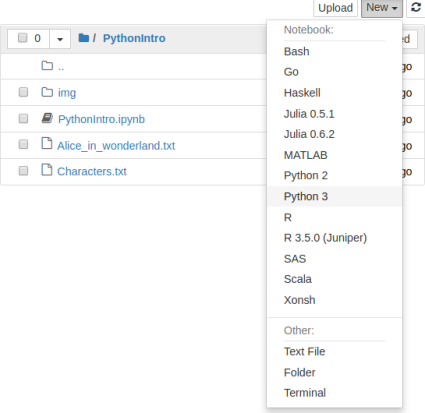
\includegraphics{Python/PythonIntro/images/notebook_new.png}
\caption{notebook\_new.png}
\end{figure}

A Jupyter Notebook contains one or more \emph{cells} containing notes or
code. To insert a new cell click the \texttt{+} button in the upper
left. To execute a cell, select it and press \texttt{Control+Enter} or
click the \texttt{Run} button at the top.

\begin{Shaded}
\begin{Highlighting}[]
\NormalTok{knitr}\OperatorTok{::}\NormalTok{opts_chunk}\OperatorTok{$}\KeywordTok{set}\NormalTok{(}\DataTypeTok{eval =} \OtherTok{FALSE}\NormalTok{, }\DataTypeTok{results =} \OtherTok{FALSE}\NormalTok{, }\DataTypeTok{message =} \OtherTok{FALSE}\NormalTok{, }\DataTypeTok{warning =} \OtherTok{FALSE}\NormalTok{, }\DataTypeTok{error =} \OtherTok{FALSE}\NormalTok{)}
\end{Highlighting}
\end{Shaded}

\section{Reading the text of Alice in Wonderland from a
file}\label{reading-the-text-of-alice-in-wonderland-from-a-file}

Reading information from a file is the first step in many projects, so
we'll start there. The workshop materials you downloaded earlier include
a file named \texttt{Alice\_in\_wonderland.txt} which contains the text
of Lewis Carroll's \emph{Alice's Adventures in Wonderland}.

We can open a connection to a file using the \emph{open} function, and
store the result using the \texttt{=} operator.

\begin{Shaded}
\begin{Highlighting}[]
\NormalTok{alice_file }\OperatorTok{=} \BuiltInTok{open}\NormalTok{(}\StringTok{"Alice_in_wonderland.txt"}\NormalTok{)}
\end{Highlighting}
\end{Shaded}

The name on the left of the equals sign (\texttt{alice\_file}) is one
that we chose. When choosing names, \emph{start with a letter}, and use
only \emph{letters}, \emph{numbers} and \emph{underscores}.

The \texttt{alice\_file} object we just created does \emph{not} contain
the contents of \texttt{Alice\_in\_wonderland.txt}. It a representation
in Python of the \emph{file itself} rather than the \emph{contents} of
the file.

The \texttt{alice\_file} object provides \emph{methods} that we can use
to do things with it. Methods are invoked using syntax that looks like
\texttt{ObjectName.method()}. You can see the methods available for
acting on an object by typing the object's name followed by a \texttt{.}
and pressing the \texttt{tab} key. For example, typing
\texttt{alice\_file.} and pressing \texttt{tab} will display a list of
methods as shown below.
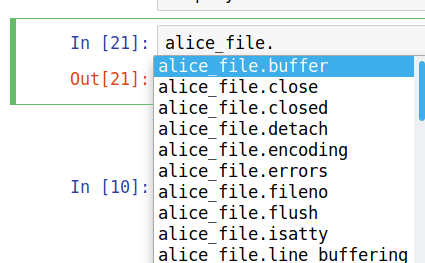
\includegraphics{Python/PythonIntro/images/notebook_file_completion.png}.

Among the methods we have for doing things with our \texttt{alice\_file}
object is one named \texttt{read}. We can use the \texttt{help} function
to learn more about it.

\begin{Shaded}
\begin{Highlighting}[]
\BuiltInTok{help}\NormalTok{(alice_file.read)}
\end{Highlighting}
\end{Shaded}

Since \texttt{alice\_file.read} looks promising, we will invoke this
method and see what it does.

\begin{Shaded}
\begin{Highlighting}[]
\NormalTok{alice_txt }\OperatorTok{=}\NormalTok{ alice_file.read()}
\BuiltInTok{print}\NormalTok{(alice_txt[:}\DecValTok{500}\NormalTok{]) }\CommentTok{# the [:500] gets the first 500 character -- more on this later.}
\end{Highlighting}
\end{Shaded}

That's all there is to it! We've read the contents of
\texttt{Alice\_in\_wonderland.txt} and stored this text in a Python
object we named \texttt{alice\_txt}. Now let's start to explore this
object, and learn some more things about Python along the way.

\section{Counting chapters, lines, and
words}\label{counting-chapters-lines-and-words}

Now that we have the text we can start answering some questions about
it. To begin with, how many words does it contain? To answer this
question we can split the text up so there is one element per word, and
then count the number of words.

\subsection{Splitting a string into a list of
words}\label{splitting-a-string-into-a-list-of-words}

How do we figure out how to split strings in Python? By asking Python
what our \texttt{alice\_txt} object is and what methods it provides. We
can ask Python what things are using the \texttt{type} function, like
this:

\begin{Shaded}
\begin{Highlighting}[]
\BuiltInTok{type}\NormalTok{(alice_txt)}
\end{Highlighting}
\end{Shaded}

Python tells us that \texttt{alice\_txt} is of type \texttt{str} (i.e.,
it is a string). We can find out what methods are available for working
strings by typing \texttt{alice\_txt.} and pressing \texttt{tab}. We'll
see that among the methods is one named \texttt{split}, as shown below.
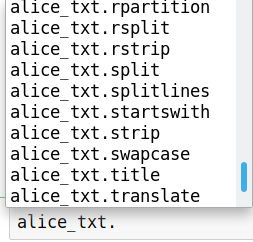
\includegraphics{Python/PythonIntro/images/notebook_string_completion.png}
To learn how to use this method we can check the documentation.

\begin{Shaded}
\begin{Highlighting}[]
\BuiltInTok{help}\NormalTok{(alice_txt.split)}
\end{Highlighting}
\end{Shaded}

Since the default is to split on whitespace (spaces, newlines, tabs) we
can get a reasonable word count simply by calling the split method and
counting the number of elements in the result.

\begin{Shaded}
\begin{Highlighting}[]
\NormalTok{alice_words }\OperatorTok{=}\NormalTok{ alice_txt.split()}
\BuiltInTok{len}\NormalTok{(alice_words)}
\end{Highlighting}
\end{Shaded}

\subsection{Using sets to calculate the number of unique
words}\label{using-sets-to-calculate-the-number-of-unique-words}

According to our computation above, there are about 26 thousand total
words in \emph{Alice's Adventures in Wonderland}. But how many
\emph{unique} words are there? Python has a special data structure
called a \emph{set} that makes it easy to find out. A \emph{set} drops
all duplicates, giving a collection of the unique elements.

\begin{Shaded}
\begin{Highlighting}[]
\BuiltInTok{len}\NormalTok{(}\BuiltInTok{set}\NormalTok{(alice_words))}
\end{Highlighting}
\end{Shaded}

There are 5295 unique words in the text.

\section{Exercise: Reading text from a file and
splitting}\label{exercise-reading-text-from-a-file-and-splitting}

\emph{Alice's Adventures in Wonderland} is full of memorable characters.
The main characters from the story are listed, one-per-line, in the file
named \texttt{Characters.txt}.

NOTE: we will not always explicitly demonstrate everything you need to
know in order to complete an exercise. Instead we focus on teaching you
how to discover available methods and how use the help function to learn
how to use them. It is expected that you will spend some time during the
exercises looking for appropriate methods and perhaps reading
documentation.

\begin{enumerate}
\def\labelenumi{\arabic{enumi}.}
\item
  Open the \texttt{Characters.txt} file and read its contents.
\item
  Split text on newlines to produce a list with one element per line.
  Store the result as ``alice\_characters''.
\end{enumerate}

```

\subsection{Working with lists}\label{working-with-lists}

The \texttt{split} methods we used to break up the text of \emph{Alice
in Wonderland} into words produced a \emph{list}. A lot of the
techniques we'll use later to analyze this text also produce lists, so
its worth taking a minute to learn more about them.

It is always a good idea to know what type of things you're working with
in Python. As you gain experience, you won't have to look this things up
as often, but even experienced Python programmers use the \texttt{type}
function to learn about the objects they are working with.

\begin{Shaded}
\begin{Highlighting}[]
\BuiltInTok{type}\NormalTok{(alice_words)}
\end{Highlighting}
\end{Shaded}

A \emph{list} in Python is used to store a collection of items. As with
other types in Python, you can get a list of methods by typing the name
of the object followed by a \texttt{.} and pressing \texttt{tab}.

\subsubsection{Extracting subsets from
lists}\label{extracting-subsets-from-lists}

Among the things you can do with a list is extract subsets using bracket
indexing notation. This is useful in many situations, including the
current one where we want to inspect a long list without printing out
the whole thing.

The examples below show how indexing works in Python.

\begin{Shaded}
\begin{Highlighting}[]
\NormalTok{alice_words[}\DecValTok{0}\NormalTok{] }\CommentTok{# first word (yes, we count from zero!)}
\end{Highlighting}
\end{Shaded}

\begin{Shaded}
\begin{Highlighting}[]
\NormalTok{alice_words[}\DecValTok{1}\NormalTok{] }\CommentTok{# second word}
\end{Highlighting}
\end{Shaded}

\begin{Shaded}
\begin{Highlighting}[]
\NormalTok{alice_words[:}\DecValTok{10}\NormalTok{] }\CommentTok{# first 10 words}
\end{Highlighting}
\end{Shaded}

\begin{Shaded}
\begin{Highlighting}[]
\NormalTok{alice_words[}\DecValTok{10}\NormalTok{:}\DecValTok{20}\NormalTok{] }\CommentTok{# words 11 through 20}
\end{Highlighting}
\end{Shaded}

\begin{Shaded}
\begin{Highlighting}[]
\NormalTok{alice_words[}\OperatorTok{-}\DecValTok{1}\NormalTok{] }\CommentTok{# the last word}
\end{Highlighting}
\end{Shaded}

\begin{Shaded}
\begin{Highlighting}[]
\NormalTok{alice_words[}\OperatorTok{-}\DecValTok{10}\NormalTok{:] }\CommentTok{# the last 10 words}
\end{Highlighting}
\end{Shaded}

Note that the displayed representation of lists and other data
structures in python often closely matches the syntax used to create
them. For example, we can create a list using square brackets, just as
we see when we print a list:

\begin{Shaded}
\begin{Highlighting}[]
\NormalTok{[}\StringTok{'her'}\NormalTok{,}
 \StringTok{'own'}\NormalTok{,}
 \StringTok{'child-life,'}\NormalTok{,}
 \StringTok{'and'}\NormalTok{,}
 \StringTok{'the'}\NormalTok{,}
 \StringTok{'happy'}\NormalTok{,}
 \StringTok{'summer'}\NormalTok{,}
 \StringTok{'days.'}\NormalTok{,}
 \StringTok{'THE'}\NormalTok{,}
 \StringTok{'END'}\NormalTok{]}
\end{Highlighting}
\end{Shaded}

\subsubsection{Sorting and other in-place
methods}\label{sorting-and-other-in-place-methods}

There are many other things we can do with lists besides extracting
subsets using bracket indexing. For example, there are methods to append
and remove elements from a list. When using a list method that you are
unfamiliar with, it is always a good idea to read the documentation.

Note that many methods modify the object \emph{in place}. For example,
if we wanted to sort the last 10 words in \texttt{alice\_words} we would
do it like this:

\begin{Shaded}
\begin{Highlighting}[]
\NormalTok{last_10 }\OperatorTok{=}\NormalTok{ alice_words[}\OperatorTok{-}\DecValTok{10}\NormalTok{:]}
\BuiltInTok{print}\NormalTok{(last_10)}
\NormalTok{last_10.sort()}
\BuiltInTok{print}\NormalTok{(last_10)}
\end{Highlighting}
\end{Shaded}

\subsection{Counting chapters and
paragraphs}\label{counting-chapters-and-paragraphs}

Now that we know how to split a string and how to work with the
resulting list, we can split on chapter markers to count the number of
chapters. All we need to do is specify the string to split on. Since
each chapter is marked with the string
\texttt{\textquotesingle{}CHAPTER\ \textquotesingle{}} followed by the
chapter number, we can split the text up into chapters using this as the
separator.

\begin{Shaded}
\begin{Highlighting}[]
\NormalTok{alice_chapters }\OperatorTok{=}\NormalTok{ alice_txt.split(}\StringTok{"CHAPTER "}\NormalTok{)}
\BuiltInTok{len}\NormalTok{(alice_chapters)}
\end{Highlighting}
\end{Shaded}

Since the first element contains the material \emph{before} the first
chapter, this tells us there are twelve chapters in the book.

We can count paragraphs in a similar way. Paragraphs are indicated by a
blank line, i.e., two newlines in a row. When working with strings we
can represent newlines with \texttt{\textbackslash{}n}, so our basic
paragraph separator is \texttt{\textbackslash{}n\textbackslash{}n}.

\begin{Shaded}
\begin{Highlighting}[]
\NormalTok{alice_paragraphs }\OperatorTok{=}\NormalTok{ alice_txt.split(}\StringTok{"}\CharTok{\textbackslash{}n\textbackslash{}n}\StringTok{"}\NormalTok{)}
\end{Highlighting}
\end{Shaded}

Before counting the number of paragraphs, I want to inspect the result
to see if it looks correct:

\begin{Shaded}
\begin{Highlighting}[]
\BuiltInTok{print}\NormalTok{(alice_paragraphs[}\DecValTok{0}\NormalTok{], }\StringTok{"}\CharTok{\textbackslash{}n}\StringTok{=========="}\NormalTok{)}
\BuiltInTok{print}\NormalTok{(alice_paragraphs[}\DecValTok{1}\NormalTok{], }\StringTok{"}\CharTok{\textbackslash{}n}\StringTok{=========="}\NormalTok{)}
\BuiltInTok{print}\NormalTok{(alice_paragraphs[}\DecValTok{2}\NormalTok{], }\StringTok{"}\CharTok{\textbackslash{}n}\StringTok{=========="}\NormalTok{)}
\BuiltInTok{print}\NormalTok{(alice_paragraphs[}\DecValTok{3}\NormalTok{], }\StringTok{"}\CharTok{\textbackslash{}n}\StringTok{=========="}\NormalTok{)}
\BuiltInTok{print}\NormalTok{(alice_paragraphs[}\DecValTok{4}\NormalTok{], }\StringTok{"}\CharTok{\textbackslash{}n}\StringTok{=========="}\NormalTok{)}
\BuiltInTok{print}\NormalTok{(alice_paragraphs[}\DecValTok{5}\NormalTok{], }\StringTok{"}\CharTok{\textbackslash{}n}\StringTok{=========="}\NormalTok{)}
\end{Highlighting}
\end{Shaded}

We're counting the title, author, and chapter lines as paragraphs, but
this will do for a rough count.

\begin{Shaded}
\begin{Highlighting}[]
\BuiltInTok{len}\NormalTok{(alice_paragraphs)}
\end{Highlighting}
\end{Shaded}

\section{Exercise: count the number of main
characters}\label{exercise-count-the-number-of-main-characters}

So far we've learned that there are 12 chapters, around 830 paragraphs,
and about 26 thousand words in \emph{Alice's Adventures in Wonderland}.
Along the way we've also learned how to open a file and read its
contents, split strings, calculate the length of objects, discover
methods for string and list objects, and index/subset lists in Python.
Now it is time for you to put these skills to use to learn something
about the main characters in the story.

\begin{enumerate}
\def\labelenumi{\arabic{enumi}.}
\item
  Count the number of main characters in the story (i.e., get the length
  of the list you created in previous exercise).
\item
  Extract and print just the first character from the list you created
  in the previous exercise.
\item
  (BONUS, optional): Sort the list you created in step 2 alphabetically,
  and then extract the last element.
\end{enumerate}

\section{Working with nested structures: words within paragraphs within
chapters}\label{working-with-nested-structures-words-within-paragraphs-within-chapters}

This far our analysis as treated the text as a ``flat'' data structure.
For example, when we counted words we just counted words in the whole
document, rather than counting the number of words in each chapter. If
we want to treat our document as a nested structure, with words forming
sentences, sentences forming paragraphs, paragraphs forming chapters,
and chapters forming the book, we need to learn some additional tools.
Specifically, we need to learn how to iterate over lists (or other
collections) and do things with each element in a collection.

There are several ways to iterate in Python, of which we will focus on
\emph{for loops} and \emph{list comprehensions}.

\subsection{Iterating over paragraphs using
for-loops}\label{iterating-over-paragraphs-using-for-loops}

A \emph{for loop} is a way of cycling through the elements of a
collection and doing something with each one. As a simple example, we
can cycle through the first 6 paragraphs and print each one. Cycling
through with a loop makes it easy to insert a separator between the
paragraphs, making it much easier to read the output.

\begin{Shaded}
\begin{Highlighting}[]
\ControlFlowTok{for}\NormalTok{ paragraph }\KeywordTok{in}\NormalTok{ alice_paragraphs[:}\DecValTok{6}\NormalTok{]:}
    \BuiltInTok{print}\NormalTok{(paragraph)}
    \BuiltInTok{print}\NormalTok{(}\StringTok{'=================================='}\NormalTok{)}
\BuiltInTok{print}\NormalTok{(}\StringTok{'DONE.'}\NormalTok{)}
\end{Highlighting}
\end{Shaded}

Notice that the syntax of a for-loop is

\begin{verbatim}
for <thing> in <collection>:
    do stuff with <thing>
\end{verbatim}

Notice also that the body of the for-loop is indented. This is
important, because it is this indentation that defines the body of the
loop. Notice that ``DONE.'' is only printed once, since
\texttt{print(\textquotesingle{}DONE.\textquotesingle{})} is not
indented and is therefore outside of the body of the loop.

Loops in Python are great because the syntax is relatively simple, and
because they are very powerful. Inside of the body of a loop you can use
all the tools you use elsewhere in python.

Here is one more example of a loop, this time iterating over all the
chapters and calculating the number of paragraphs in each chapter.

\begin{Shaded}
\begin{Highlighting}[]
\ControlFlowTok{for}\NormalTok{ chapter }\KeywordTok{in}\NormalTok{ alice_chapters[}\DecValTok{1}\NormalTok{:]:}
\NormalTok{    paragraphs }\OperatorTok{=}\NormalTok{ chapter.split(}\StringTok{"}\CharTok{\textbackslash{}n\textbackslash{}n}\StringTok{"}\NormalTok{)}
    \BuiltInTok{print}\NormalTok{(}\BuiltInTok{len}\NormalTok{(paragraphs))}
\end{Highlighting}
\end{Shaded}

\subsection{Iterating and collecting paragraphs per chapter using list
comprehension}\label{iterating-and-collecting-paragraphs-per-chapter-using-list-comprehension}

We could use for-loops to fill in lists of values, but there is a
special syntax in Python that is often better for this use case. This
special syntax is called a \emph{list comprehension} and it looks like
this:

\begin{Shaded}
\begin{Highlighting}[]
\NormalTok{paragraphs_per_chapter }\OperatorTok{=}\NormalTok{ [}\BuiltInTok{len}\NormalTok{(chapter.split(}\StringTok{"}\CharTok{\textbackslash{}n\textbackslash{}n}\StringTok{"}\NormalTok{)) }
                          \ControlFlowTok{for}\NormalTok{ chapter }\KeywordTok{in}\NormalTok{ alice_chapters[}\DecValTok{1}\NormalTok{:]]}
\BuiltInTok{print}\NormalTok{(paragraphs_per_chapter)}
\end{Highlighting}
\end{Shaded}

Notice that \emph{list comprehension} is very similar to a \emph{for
loop}, though the order is different. In a \emph{for-loop} the
\texttt{for} part comes first and the expressions that make up the body
come second and are indented. In a \emph{list comprehension} the
expression comes first and the \texttt{for} part comes afterward. Notice
also the square brackets surrounding the whole thing -- these brackets
are what tells Python that you want a list.

Here is another list comprehension that counts the number of times the
name ``Alice'' appears in each chapter.

\begin{Shaded}
\begin{Highlighting}[]
\NormalTok{alices_per_chapter }\OperatorTok{=}\NormalTok{ [chapter.count(}\StringTok{"Alice"}\NormalTok{) }\ControlFlowTok{for}\NormalTok{ chapter }\KeywordTok{in}\NormalTok{ alice_chapters]}
\BuiltInTok{print}\NormalTok{(alices_per_chapter)}
\end{Highlighting}
\end{Shaded}

\subsection{Organizing results in
dictionaries}\label{organizing-results-in-dictionaries}

Our code for calculating the number of of times ``Alice'' was mentioned
per chapter worked, but with a little effort we can make it much easier
to interpret by associating each count with the chapter it corresponds
to. In Python we can use a \texttt{dict} (i.e., ``dictionary'') to store
key-value pairs.

First, we can iterate over each chapter and grab just the first line
(that is, the chapter titles). These will become our keys.

\begin{Shaded}
\begin{Highlighting}[]
\NormalTok{chapter_names }\OperatorTok{=}\NormalTok{ [chapter.splitlines()[}\DecValTok{0}\NormalTok{] }\ControlFlowTok{for}\NormalTok{ chapter }\KeywordTok{in}\NormalTok{ alice_chapters[}\DecValTok{1}\NormalTok{:]]}
\BuiltInTok{print}\NormalTok{(chapter_names)}
\end{Highlighting}
\end{Shaded}

Finally we can combine the chapter titles and counts and convert them to
a dictionary.

\begin{Shaded}
\begin{Highlighting}[]
\BuiltInTok{dict}\NormalTok{(}\BuiltInTok{zip}\NormalTok{(chapter_names, }
\NormalTok{         [chapter.count(}\StringTok{"Alice"}\NormalTok{) }
          \ControlFlowTok{for}\NormalTok{ chapter }\KeywordTok{in}\NormalTok{ alice_chapters]))}
\end{Highlighting}
\end{Shaded}

\section{Exercise: Iterating and counting
things}\label{exercise-iterating-and-counting-things}

Now that we know how to iterate using for-loops and list comprehensions
the possibilities really start to open up. For example, we can use these
techniques to count the number of times each character appears in the
story.

\begin{enumerate}
\def\labelenumi{\arabic{enumi}.}
\tightlist
\item
  Make sure you have both the text and the list of characters.
\end{enumerate}

Open and read both ``Alice\_in\_wonderland.txt'' and ``Characters.txt''
if you have not already done so.

\begin{enumerate}
\def\labelenumi{\arabic{enumi}.}
\setcounter{enumi}{1}
\tightlist
\item
  Which chapter has the most words?
\end{enumerate}

Split the text into chaptes (i.e., split on ``CHAPTER'') and use a
for-loop or list comprehension to iterate over the chapters. For each
chapter, split it into words and calculate the length.

\begin{enumerate}
\def\labelenumi{\arabic{enumi}.}
\setcounter{enumi}{2}
\tightlist
\item
  How many times is each character mentioned in the text?
\end{enumerate}

Iterate over the list of characters using a for-loop or list
comprehension. For each character, call the count method with that
character as the argument.

\begin{enumerate}
\def\labelenumi{\arabic{enumi}.}
\setcounter{enumi}{3}
\tightlist
\item
  (BONUS, optional): Put the character counts computed above in a
  dictionary with character names as the keys and counts as the values.
\item
  (BONUS, optional): Use a nested list comprehension to calculate the
  number of times each character is mentioned in each chapter.
\end{enumerate}

\section{Importing numpy and calculating simple
statistics}\label{importing-numpy-and-calculating-simple-statistics}

Now that we know how to iterate over lists and calculate numbers for
each element, we may wish to do some simple math using these numbers.
For example, we may want to calculate the mean and standard deviation of
the distribution of the number of paragraphs in each chapter. Python has
a handful of math functions built-in (e.g., \texttt{min} and
\texttt{max}) but built-in math support is pretty limited.

When you find that something isn't available in Python itself, its time
to look for a package that does it. Although it is somewhat overkill for
simply calculating a mean we're going to use a popular package called
\emph{numpy} for this. The \emph{numpy} package is included in the
Anaconda Python distribution we are using, so we don't need to install
it separately.

In order to use \emph{numpy} or other packages, you must first import
them. We can import numpy as follows:

\begin{Shaded}
\begin{Highlighting}[]
\ImportTok{import}\NormalTok{ numpy}
\end{Highlighting}
\end{Shaded}

The \emph{numpy} package is very popular and includes a lot of useful
functions. For example, we can use it to calculate means and standard
deviations:

\begin{Shaded}
\begin{Highlighting}[]
\BuiltInTok{print}\NormalTok{(numpy.mean(paragraphs_per_chapter))}
\BuiltInTok{print}\NormalTok{(numpy.std(paragraphs_per_chapter))}
\end{Highlighting}
\end{Shaded}

and compute correlations:

\begin{Shaded}
\begin{Highlighting}[]
\NormalTok{words_per_chapter }\OperatorTok{=}\NormalTok{ [}\BuiltInTok{len}\NormalTok{(chapter.split()) }\ControlFlowTok{for}\NormalTok{ chapter }\KeywordTok{in}\NormalTok{ alice_chapters]}
\NormalTok{alices_per_chapter }\OperatorTok{=}\NormalTok{ [chapter.count(}\StringTok{"Alice"}\NormalTok{) }\ControlFlowTok{for}\NormalTok{ chapter }\KeywordTok{in}\NormalTok{ alice_chapters]}

\BuiltInTok{print}\NormalTok{(numpy.corrcoef(words_per_chapter, alices_per_chapter))}
\end{Highlighting}
\end{Shaded}

\section{Where to go from here}\label{where-to-go-from-here}

By this time you've learned a lot about python, including how to read
files, call functions, lookup and use methods, process text, manipulate
lists and dictionaries, and iterate using loops and comprehensions.
There is more to learn, but you probably know enough already to be
dangerous. Your next steps are to a) keep learning Python basics and b)
find and learn how to use packages that help you accomplish your
substantive goals.

Here are some packages you might be interested in learning:

\begin{itemize}
\tightlist
\item
  Graphics

  \begin{itemize}
  \tightlist
  \item
    \href{https://matplotlib.org/}{matplotlib}
  \item
    \href{https://seaborn.pydata.org/}{seaborn}
  \item
    \href{https://plot.ly/python/}{plotly}
  \end{itemize}
\item
  Quantitative Data Analysis

  \begin{itemize}
  \tightlist
  \item
    \href{http://www.numpy.org/}{numpy}
  \item
    \href{https://www.scipy.org/}{scipy}
  \item
    \href{https://pandas.pydata.org/}{pandas}
  \item
    \href{http://scikit-learn.org/stable/}{scikit-learn}
  \item
    \href{http://www.statsmodels.org/stable/}{statsmodels}
  \end{itemize}
\item
  Text analysis

  \begin{itemize}
  \tightlist
  \item
    \href{https://textblob.readthedocs.io/en/dev/}{textblob}
  \item
    \href{http://www.nltk.org/}{nltk}
  \item
    \href{https://radimrehurek.com/gensim/}{Gensim}
  \end{itemize}
\item
  Webscraping

  \begin{itemize}
  \tightlist
  \item
    \href{https://scrapy.org/}{scrapy}
  \item
    \href{http://docs.python-requests.org/en/master/}{requests}
  \item
    \href{https://lxml.de/}{lxml}
  \item
    \href{https://www.crummy.com/software/BeautifulSoup/}{BeautifulSoup}
  \end{itemize}
\item
  Social Network Analysis

  \begin{itemize}
  \tightlist
  \item
    \href{https://networkx.github.io/}{networkx}
  \item
    \href{https://graph-tool.skewed.de/}{graph-tool}
  \end{itemize}
\end{itemize}


\end{document}
